\documentclass[a4paper,11pt]{article}
\usepackage[utf8]{inputenc}
\usepackage{graphicx}
\usepackage{graphicx}
\usepackage{amsmath}
\usepackage[spanish, es-nodecimaldot]{babel}
\usepackage[
	left=2.5cm,
	right=2.5cm,
	top=2cm,
	bottom=2cm
]{geometry}
\begin{document}
\pagestyle{empty}
\begin{center}
	\vspace*{3cm}
	\Huge{Tecnológico Nacional de México}
	
	\vspace{0.2cm}
	\huge{Instituto Tecnológico de Tijuana}
	
	\vspace{0.2cm}
	\Large{Maestría en Ciencias de la Computación}
	
	\vspace{2cm}
	\LARGE{Control para Sistemas de Calentamiento Hidrónico Multizona usando Lógica Difusa y Algoritmos Bio-Inspirados}
	
	\vspace{1.5cm}
	\LARGE{Tesis}
	
	\vspace{1cm}
	\footnotesize{Para Obtener el Título de}
	
	\Large{Maestro en Ciencias de la Computación}
	
	\vspace{1cm}
	\footnotesize{Presenta}

	\normalsize{Ing. Ian Alfonso Ruiz Naranjo}
	
	\vspace{1cm}
	\footnotesize{Director}
	
	\normalsize{Dr. Mario García Valdez}
	
	\vspace{0.4cm}
	\footnotesize{Codirector}
	
	\normalsize{Dr. Oscar Castillo}
	
	\vspace{1cm}
	\small{Tijuana, Baja California, México}
\end{center}
\pagestyle{empty}
\begin{center}
	\vspace*{\fill}
	\textit{A mi papá Alfonso, a mi mamá Julia, a mi hermano Alejandro, a mi amor Itzel, a la princesa Nara y a el travieso Pichu.}
	\vspace*{\fill}
\end{center}
\tableofcontents
\include{./TeX_files/introduccion}
\section{Objetivo General}

Crear un controlador predictivo para sistemas de calentamiento hidrónico usando lógica difusa y algoritmos bio-inspirados entrenado en un simulador computacional basado en leyes termo-físicas que contiene modelos de fenómenos de transferencia de calor de sus componentes, así como de condiciones atmosféricas, solares y de ocupación habitacional.
\section{Objetivos Específicos}

\begin{itemize}
	\item Implementar modelos de transferencia de calor para los componentes que conforman el espacio habitacional que se busca acondicionar térmicamente.
	\item Implementar un modelo de predicción atmosférica utilizando redes neuronales recurrentes.
	\item Implementar un modelo de predicción de irradiación solar, así como de geometría solar para determinar cargas térmicas.
	\item Implementar un modelo de predicción de ocupación habitacional.
	\item Implementar algoritmos bio-inspirados para ser consumidos por el proceso de optimización del controlador.
	\item Desarrollar un simulador de un sistema hidrónico e integrar los modelos predictivos para enriquecer el proceso de optimización del controlador difuso.
	\item Implementar el simulador, así como todas las dependencias y/o resultantes en el lenguaje de programación en Python y diferentes variantes.
\end{itemize}
\section{Problemática}
\section{Estado del Arte}
\section{Marco Teórico}

\subsection{Radiacón Solar}

\subsubsection{El Sol}

\subsubsection{La Constante Solar}
La tierra tiene una órbita elíptica cuya excentricidad es tal que la distancia entre la tierra y el sol varía un 1.7\%. Debido a que la variación es pequeña, la cantidad de radiación emitida por el sol es casi fija fuera de la atmósfera terrestre. Esta energía es conocida como la constante solar $G_{sc}$, puede decirse que es la cantidad de energía del sol recibida en un área perpendicular a la dirección de propagación del haz por una unidad de tiempo.

\subsubsection{Distribución Espectral de Radiación Extraterrestre}

\subsubsection{Variación de Radiación Extraterrestre}
Cuando se estudian las variaciones de radiación extraterrestre, es necesario tomar en consideración la energía emitida por el sol. Se han identificado diferentes periodicidades y variaciones de intensidad, asociadas con la actividad de manchas solares. \\

También es necesario tomar en cuenta el impacto que tiene la órbita elíptica de la tierra con respecto al sol, la distancia entre estos dos varía causando una variación en el flujo de radiación solar en el rango del $\pm3.3\%$ \\

Existen dos modelos frecuentemente usados para calcular esta variación, el primero es razonablemente bueno para aplicaciones poco rigurosas o cotidianas, este modelo es descrito a través de la siguiente ecuación,

\begin{equation}
		G_{on} = G_{sc}\left(1 + 0.033 \cos \frac{360n}{365}\right) 
\end{equation}

Si se necesita más precisión, la siguiente expresión ofrece un $\pm0.01\%$ de variación,

\begin{align}
	\begin{aligned} \label{eq:variacion_extraterrestre_precisa}
		G_{on} & = G_{sc} \left(1.000110 + 0.034221 \cos B + 0.001280 \sin B \right.	\\
		& \left. + 0.000719 \cos 2B + 0.000077 \sin 2B \right)
	\end{aligned}
\end{align}

en dónde $G_{on}$ es la radiación incidente en el plano normal a la radiación dado un día $n$ del año. $B$ está dado por,

\begin{equation}
	B = \left(n - 1\right) \frac{360}{365}
\end{equation}

Usando la ecuación \ref{eq:variacion_extraterrestre_precisa}, obtenemos la siguiente gráfica.

\begin{figure}[htbp]
	\centering
	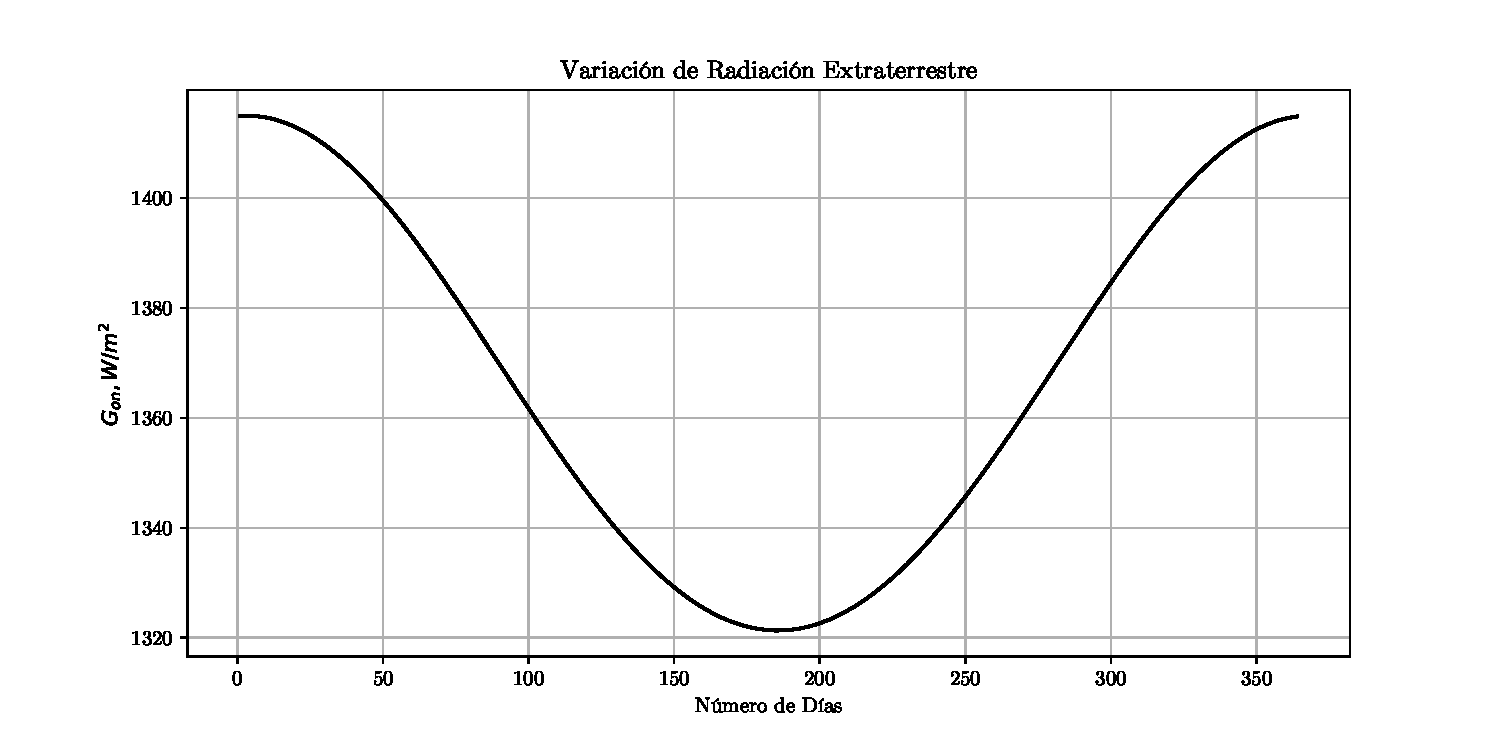
\includegraphics[width=0.8\textwidth, angle=0]{images/variationextraterrestrialsolarradiation.pdf}
	\caption{Variación de radiación solar extraterrestre en el plazo de un año.}
\end{figure}

\subsubsection{Estimación de Radiación Solar Terrestre}
Cuando la radiación solar llega a la tierra, esta tiene que pasar por una densa y grande atmósfera. En el proceso la energía toma diferentes caminos reduciendo la cantidad de energía directa que llega a la superficie terrestre. Una parte de ella es reflejada de vuelta al espacio, otra parte es absorbida por el aire y vapor de agua, otra gran parte se dispersa por moléculas de aire seco, vapor de agua, aerosoles y partículas de polvo. Todo este proceso se muestra gráficamente a continuación.

\begin{figure}[H]
	\centering
	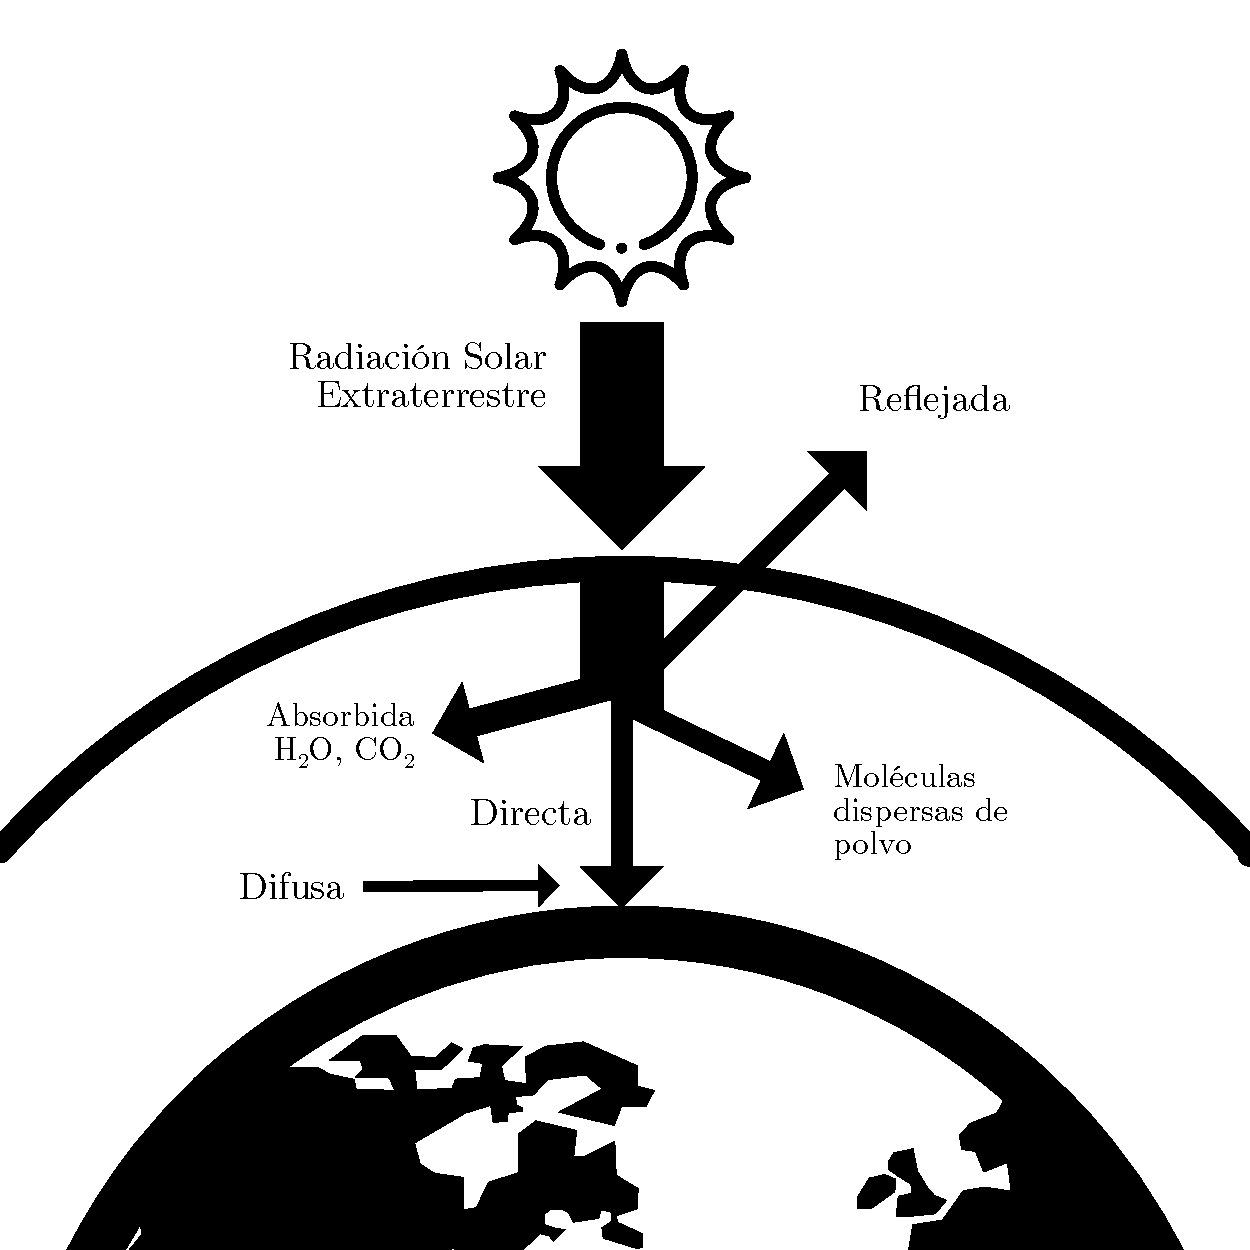
\includegraphics[width=0.5\textwidth, angle=0]{images/attenuationofsolarradiation.pdf}
	\caption{Atenuación de radiación solar.}
\end{figure}

A pesar de que la radiación extraterrestre es predecible con cierto grado de certidumbre, los niveles de radiación solar que alcanzan la tierra y entran en su atmósfera se ven sujetos a una cantidad razonable de incertidumbre debido a las interacciones climáticas locales. La información más útil proviene de bases de datos de mediciones de largo plazo, en la que los valores son promedios de esa ubicación en específico. Desafortunadamente hay ciertas regiones del mundo de las que no se tienen registros suficientemente precisos, sin embargo, en la actualidad hay más iniciativas que motivan la adquisición de esta información.

\subsubsection{Dirección del Haz de Radiación}

Las relaciones geométricas de cualquier plano con respecto a cualquier orientación relativa a la tierra, en cualquier momento y un haz entrante de radiación solar, pueden ser descritas por varios ángulos, estos por convención son nombrados y se hace referencia hacia ellos como se muestra a continuación,

\begin{itemize}
	\item $\phi$ \textbf{Latitud}, es la ubicación angular al norte o sur del ecuador, siendo la dirección del norte positiva; $-90^\circ\leq\phi\leq90^\circ$.
	\item $\delta$ \textbf{Declinación}, es la posición angular del sol al medio día solar con respecto al plano del ecuador, por ejemplo, cuando este se encuentra en la meridiana local. Esta es positiva al norte; $-23.45^\circ\leq\delta\leq23.45^\circ$.
	\item $\beta$ \textbf{Pendiente}, es el ángulo entre el plano de la superficie en cuestión y la superficie; $0^\circ\leq\beta\leq180^\circ$.
	\item $\gamma$ \textbf{Ángulo de Acimut de Superficie}, es la desviación de la proyección en un plano horizontal a la superficie desde la meridiana local. $-180.0^\circ\leq\gamma\leq180.0^\circ$.
	\item $\omega$ \textbf{Ángulo de Hora}, el desplazamiento angular del sol del este o el oeste con respecto a la meridiana local debido a la rotación de la tierra cuyo valor es de $15^\circ$ por hora; En la mañana es negativo y en el atardecer positivo.
	\item $\theta$ \textbf{Ángulo de Incidencia}, es el ángulo entre el haz de radiación en una superficie y la normal de esa superficie.
	\item $\theta_z$ \textbf{Ángulo Cenital}, es el ángulo entre la vertical y la línea hacia el sol, en otras palabras, es el ángulo de incidencia del haz de radiación en una superficie horizontal.
	\item $\alpha_s$ \textbf{Ángulo de Altitud Solar}, es el ángulo entre la horizontal y la línea hacia el sol, es el complemento del ángulo cenital.
	\item $\gamma_s$ \textbf{Ángulo de Acimut Solar}, es el desplazamiento angular del sur de la proyección del haz de radiación en un plano horizontal. Los desplazamientos del este al sur son negativos y del oeste al sur son positivos.	
\end{itemize}

\begin{figure}[htbp]
	\centering
	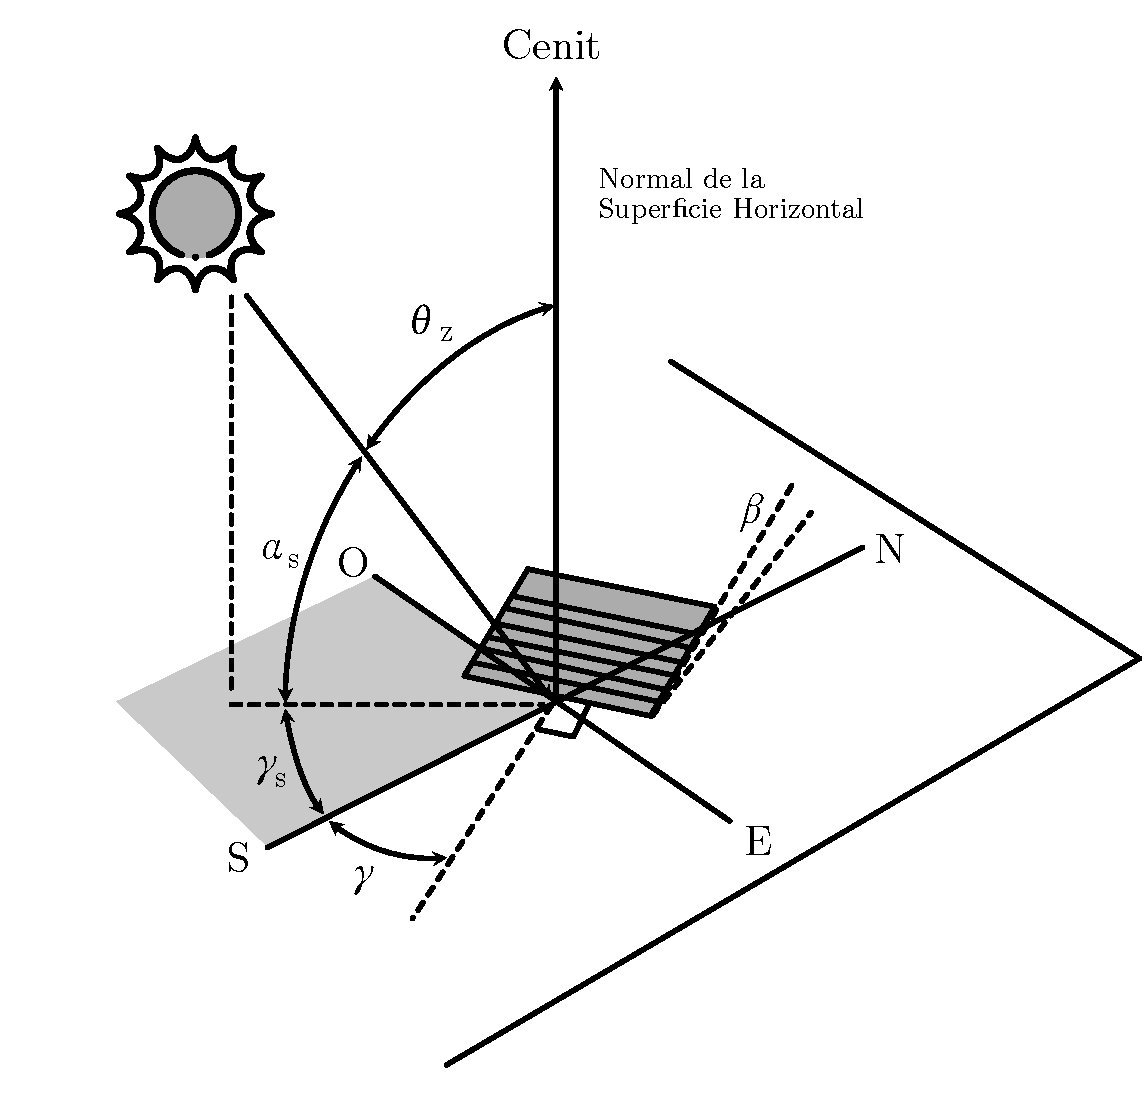
\includegraphics[width=0.6\textwidth, angle=0]{images/solarradiationdirectionangles.pdf}
	\caption{Ángulos de radiación solar.}
\end{figure}

\paragraph{La Declinación $\delta$}
Este ángulo puede ser encontrado a través de una aproximación como la que se muestra a continuación,
\begin{equation} \label{eq:declinacion_ingenieria}
\delta = 23.45 \sin\left( \frac{360}{365}\left( 284 + n\right) \right) 
\end{equation}
Para fines de ingeniería, la aproximación anterior resulta suficiente, sin embargo disponemos de otro modelo cuya precisión es mayor ya que el error es menor al $0.035^\circ$.

\begin{align} \label{eq:declinacion_precisa}
	\begin{aligned}
		\delta & = 0.006918 - 0.399912\cos\left(\Gamma \right) + 0.070257\sin(\Gamma) \\
		& -0.006758\cos\left(2\Gamma \right)  + 0.000907\sin\left(2\Gamma \right)  \\
		& -0.002697\cos\left(3\Gamma \right) + 0.00148\sin\left(3\Gamma \right)
	\end{aligned}
\end{align}

en dónde,
\begin{equation}
\Gamma = \frac{2\pi\left(n-1 \right) }{365}
\end{equation}

En ambas expresiones la variable $n$ es el número del día del año que se estudia, esta satisface $1\leq n \leq 365$.

\begin{figure}[htbp]
	\centering
	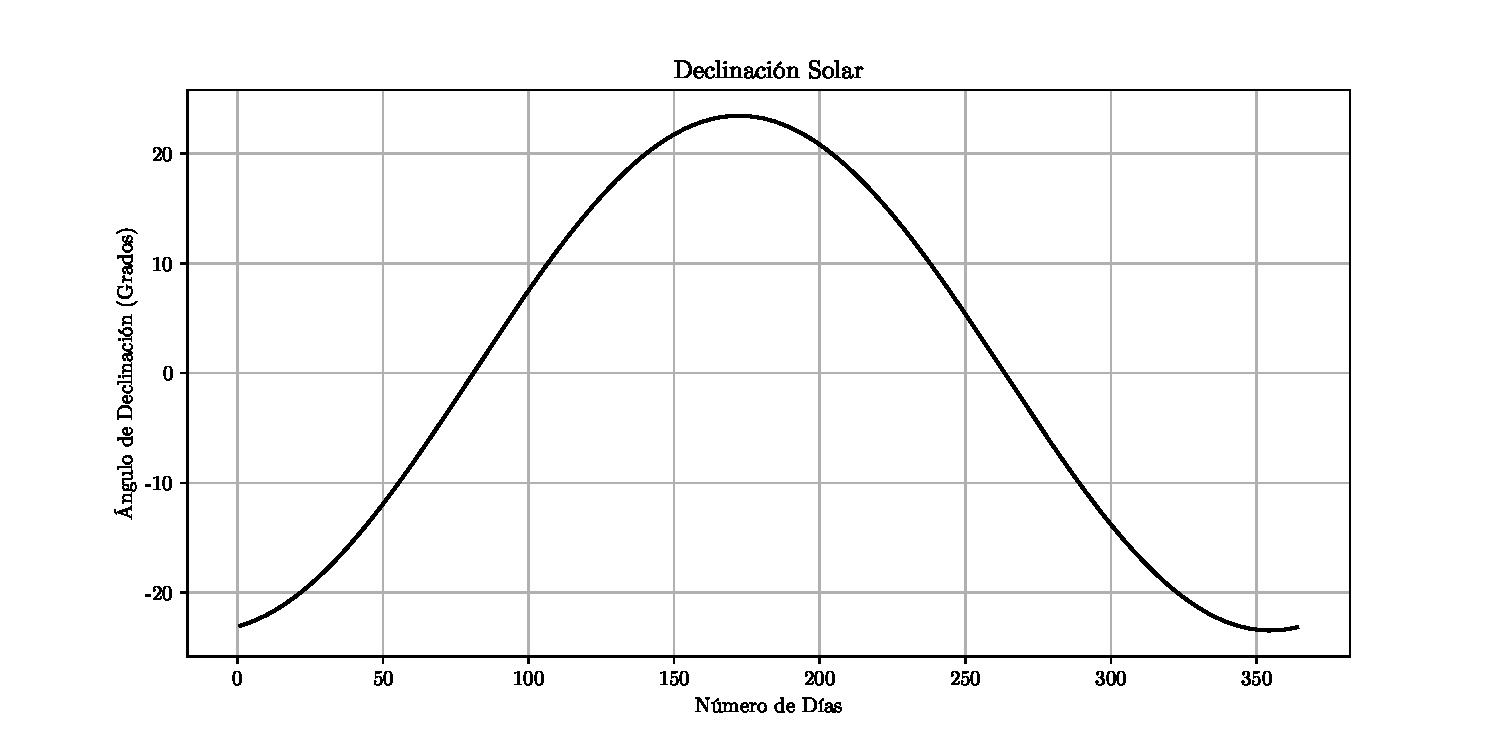
\includegraphics[width=0.8\textwidth, angle=0]{images/solardeclination.pdf}
	\caption{Diagrama de declinación solar.}
\end{figure}

Observando la interacción y dependencias entre ángulos, podemos deducir las siguientes relaciones que podemos utilizar para efectuar nuestros cálculos de posición.

\begin{align}
	\begin{aligned}
		\cos\theta & = \sin \delta \sin \phi \cos \beta - \sin \delta \cos \phi \cos \gamma \\
		& + \cos \delta \cos \phi \cos \beta \cos \omega + \cos \delta \sin \phi \sin \beta \cos \gamma \cos \omega \\
		& + \cos \delta \sin \beta \sin \gamma \sin \omega
	\end{aligned}
\end{align}
Y la siguiente expresión,
\begin{align}
	\begin{aligned}
		\cos\theta & = \cos \theta_z \cos \beta + \sin \theta_z \sin \beta \cos\left(\gamma_s - \gamma \right) 
	\end{aligned}
\end{align}

El ángulo $\theta$ puede exceder $90^\circ$, lo cuál significa que el sol se encuentra detrás de la superficie. \\

Con las relaciones expuestas anteriormente, se puede entonces tener un rastreo preciso de la posición del sol con respecto a un punto en la tierra usando la latitud y el día del año en el que se decide hacer la evaluación.
\section{Propuesta}
\end{document}